\documentclass[11pt,twoside,openleft]{book}
\usepackage{parskip}
\usepackage{graphicx}
\usepackage{multicol}
\usepackage{geometry}
\geometry{
    letterpaper,
    left=0.5in,
    right=0.5in,
    top=0.75in,
    bottom=0.5in,
}
\setlength{\textwidth}{7.3in}

\usepackage{titletoc}
\usepackage{titlesec}
\usepackage{lscape}
\usepackage{longtable}
\usepackage{float}
\usepackage[hidelinks,bookmarks,bookmarksdepth=2]{hyperref}

% Checklist
\usepackage{enumitem,amssymb}
\newlist{fixlist}{itemize}{2}
\setlist[fixlist]{label=$\square$}
\usepackage{pifont}
\newcommand{\cmark}{\ding{51}}%
\newcommand{\xmark}{\ding{55}}%
\newcommand{\checked}{\rlap{$\square$}{\raisebox{2pt}{\large\hspace{1pt}\cmark}}%
\hspace{-2.5pt}}
\newcommand{\needfix}{\rlap{$\square$}{\large\hspace{1pt}\xmark}}

\renewcommand{\chaptermark}[1]{\markboth{\MakeUppercase{#1}}{}}

%-- Need to find a better solution than this for chapter pages
\titleformat{\chapter}[display]
{\normalfont\Large\filcenter}
{\vspace*{\fill}
 \titlerule[1pt]%
 \vspace{1pt}%
 \titlerule
 \vspace{1pc}%
 \LARGE\MakeUppercase{}~\thechapter}
{1pc}
{\titlerule\Huge}[]


%-- Deal with unicode accents in text
\include{unicode_accents}
\DeclareGraphicsExtensions{001.eps}

\setlength{\parindent}{0pt}


% -----

\begin{document}
\pagenumbering{roman}


\title{\textbf{\Huge{The\\ 
City Pipeband Collection }}\\
of Competition Tunes}

\author{Collected and Compiled by\\Pipe Major Smith}

\date{\today\\\textit{Review Copy}}

\maketitle

\tableofcontents
\cleardoublepage
\pagenumbering{arabic}

% -----

% \newpage
\chapter{Marches}
\vspace*{\fill}\newpage

\addcontentsline{toc}{section}{Example March}
    \includegraphics[width=7.5in]{tunes/marches/example_march001.eps}

% ------------------------------------------------------------------

\cleardoublepage
\chapter{Jigs}
\vspace*{\fill}\newpage

\addcontentsline{toc}{section}{Example Jig}
\addcontentsline{toc}{section}{Alternate Title}
    \includegraphics[width=7.5in]{tunes/jigs/example_jig001.eps}


% ------------------------------------------------------------------


\cleardoublepage
\chapter{Piobaireachd}
\vspace*{\fill}\newpage


\addcontentsline{toc}{section}{Example Piobaireachd}
\addcontentsline{toc}{section}{Gaelic Title}
    \includegraphics[width=7.5in]{tunes/piobaireachd/example_piobaireachd001.eps}
    \cleardoublepage
    \includegraphics[width=7.5in]{tunes/piobaireachd/example_piobaireachd002.eps}
    \begin{center}
    \includegraphics[]{tunes/piobaireachd/example_piobaireachd003.eps}
    \end{center}

% ------------------------------------------------------------------


\cleardoublepage
\chapter{Sets}
\vspace*{\fill}\newpage

\begin{tabular}{ l l l l}
  \textbf{Name} & \textbf{Tunes} & \textbf{Instr.} & \textbf{Type}\\
  \hline
    & & & \\
Irish Set & The Minstrel Boy & & Marches\\
        & The Wearing o’ the Green & &\\
        \\
March Set & Walter Douglas MBE & & 2/4 Marches\\
        & Corriechoillie’s Welcome To The Northern Meeting & &\\
        & Teribus & &\\
        \\
Air Set & Loch Duich & & Marches\\
        & Loch Rannoch & &\\
        & Mo Dhachaidh (My Home) & &\\
        \\
Cape Breton 2/4 Set & Welcome to the Trossacks & & 2/4 Marches\\
        & Father Eugene's Welcome to Cape North & &\\
        & Trip to Mabou Ridge & &\\
        \\
Our Fevorite MSR & Donald MacLean's Farewell to Oban & & MSR\\
                   & Devil in the Kitchen & &\\
                   & Mrs MacLeod of Raasay & &\\
                   \\
\end{tabular}

\cleardoublepage
\chapter{Dance Sets}
\vspace*{\fill}\newpage

\begin{tabular}{ l l l l}
  \textbf{Name} & \textbf{Tunes} & \textbf{Instr.} & \textbf{Type}\\
  \hline

Gay Gordons: & Flett from Flotta & & Marches\\ 
             & Duncan Gray & &\\
             & The Soldiers Return & &\\
             & The Wee Highland Laddie & &\\
             & Flett from Flotta & &\\
             \\
Strip the Willow: & The Atholl Highlanders & & Marches\\
                  & The Heights of Mount Kenya & &\\
                  & Piobaireachd of Donald Dhu & &\\
                  & The Atholl Highlanders & &\\
                  \\
The Dashing White Sergeant: & The Barren Rocks of Aden & & Marches\\
                            & The High Road to Linton & &\\
                            & The Brown Haired Maid & &\\
                            & Teribus & &\\
                            & The Barren Rocks of Aden & &\\
                            \\

\end{tabular}

\cleardoublepage
\chapter{Band History or other instructional material}
\vspace*{\fill}\newpage
\chapter{Band History\\
By Pipe Major Smith\\
with forward by}

\section*{Introduction}

Lorem ipsum dolor sit amet, consectetur adipiscing elit. Curabitur purus diam, rutrum ut vestibulum sed, semper quis metus. Etiam at est arcu. Donec nulla diam, accumsan nec urna eu, consectetur ultrices lacus. Donec lorem augue, tempus eget molestie ac, tincidunt eu leo. Nulla facilisi. Nulla auctor massa eget convallis elementum. Donec vulputate nisl nec ipsum commodo vehicula quis non nisi. Curabitur sed mauris lorem. Aliquam sed sodales tortor. Suspendisse potenti. Nunc gravida vitae quam viverra ullamcorper. Nulla dignissim, ipsum nec viverra rutrum, quam orci ultricies neque, nec pulvinar nibh urna sed massa. Praesent euismod mollis vulputate. Orci varius natoque penatibus et magnis dis parturient montes, nascetur ridiculus mus. Nullam sagittis lobortis magna. Curabitur rhoncus fringilla risus sit amet viverra.

Aliquam ultricies orci vel neque auctor, in iaculis quam tincidunt. Curabitur aliquet dictum diam at congue. Aliquam porta arcu quis sapien venenatis placerat. Curabitur eget sem eu est mollis faucibus. Curabitur purus nisi, accumsan at risus eget, mollis aliquet mi. Mauris gravida tellus nec lectus bibendum tempus. Phasellus mi purus, viverra vitae lectus vitae, accumsan pharetra nisi. Nulla ante diam, placerat in dui in, lobortis pulvinar nunc. Quisque at est enim. Ut blandit quam urna. Etiam quis dui est. Quisque ultrices tortor tincidunt urna varius, a eleifend nulla egestas. 

\section*{Early Days}

Nam quis quam eu diam pellentesque dictum. Ut porttitor, enim id dignissim vestibulum, lacus nibh condimentum velit, in auctor risus sem eget elit. Nulla eu laoreet magna. In ut felis nisl. Suspendisse eu feugiat eros. Nullam non eros tristique ex aliquam congue. Donec sed augue tincidunt, lobortis ipsum in, efficitur libero. Phasellus dictum lectus luctus dui feugiat, eget hendrerit lacus blandit. Etiam finibus metus eget purus consequat euismod. Sed tristique ligula iaculis, condimentum mi et, aliquam purus. Vestibulum faucibus interdum ligula et egestas. Duis lacinia luctus semper.

Mauris at nunc tellus. Nulla ultricies placerat pellentesque. Donec consequat massa nec risus commodo dignissim non ut mi. Integer suscipit fermentum scelerisque. Morbi dapibus dignissim elit eu mollis. Maecenas eget suscipit nisi. Proin interdum blandit libero, sit amet tempus augue euismod suscipit. Etiam nec nisl sit amet mi pellentesque ultrices vel ut ex. Nulla facilisi. Ut in egestas lectus. Nam viverra lorem vel dignissim ultricies. Nulla facilisi. Quisque nec hendrerit tortor. 



% ---- Optional section to create lined paper and staves for taking notes

\cleardoublepage
\chapter{Notes}
\vspace*{\fill}\newpage

\includegraphics[width=7.5in]{graphics/notepaper.eps}


\includegraphics[width=7.5in]{graphics/notepaper.eps}

\includegraphics[width=7.5in]{graphics/notepaper.eps}


\includegraphics[width=7.5in]{graphics/notepaper.eps}

\includegraphics[width=7.5in]{graphics/notepaper.eps}


\includegraphics[width=7.5in]{graphics/notepaper.eps}

\includegraphics[width=7.5in]{graphics/notepaper.eps}


\begin{figure}
\centering
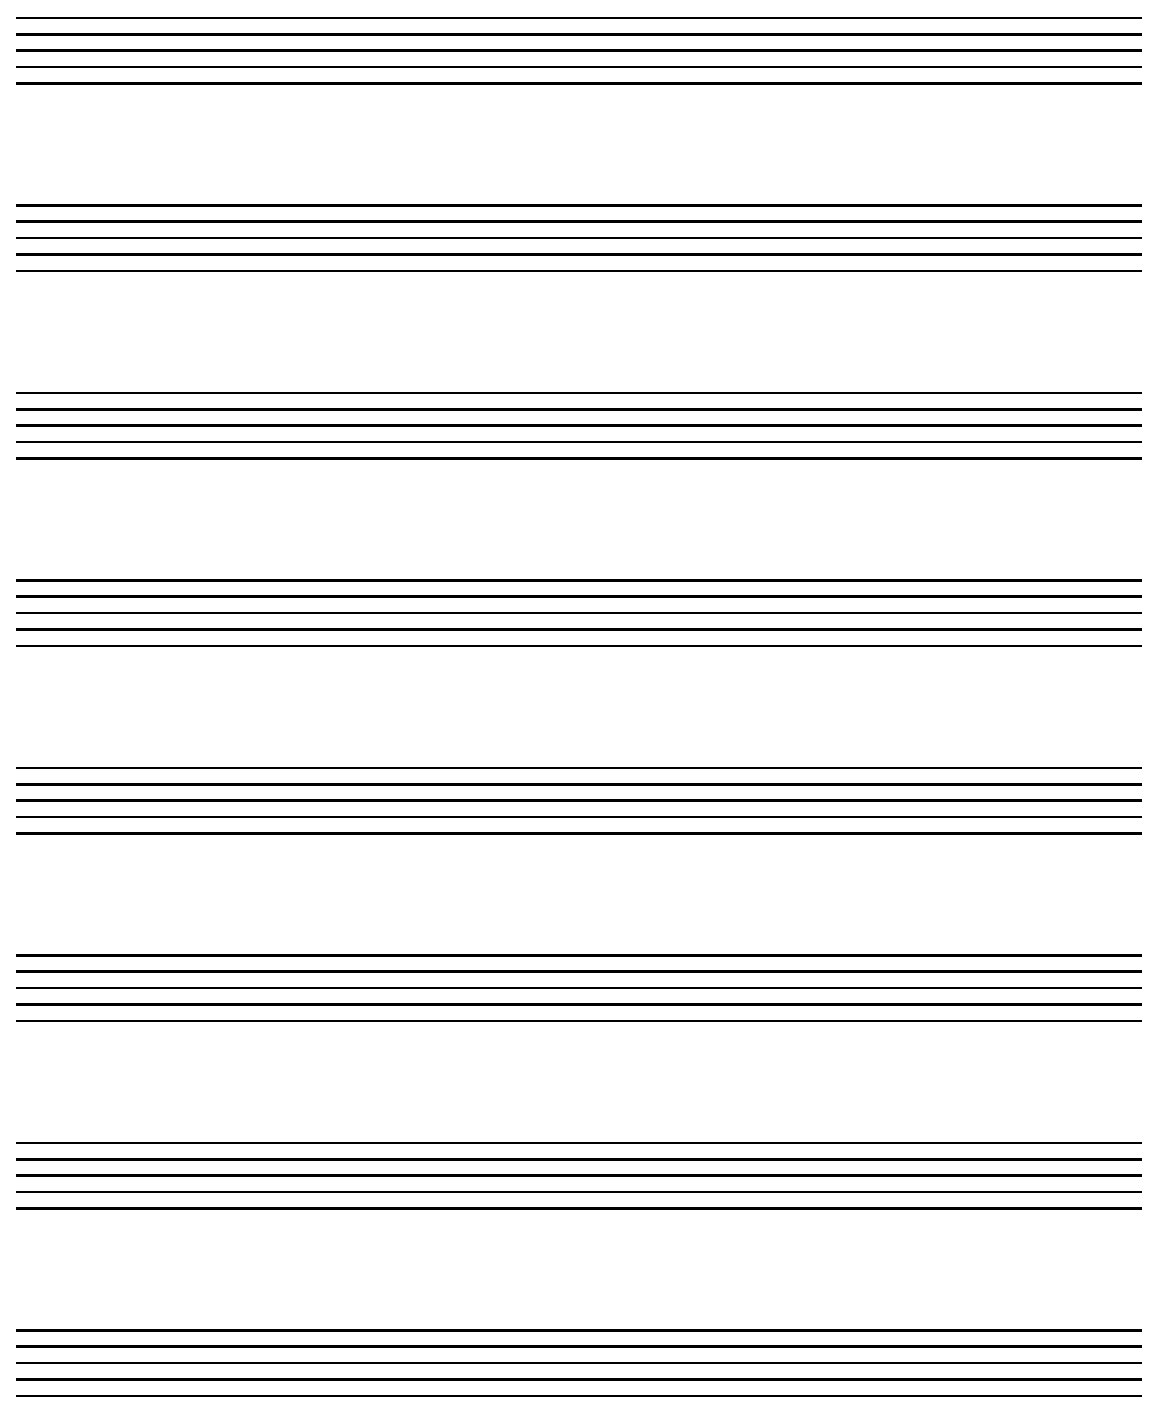
\includegraphics[width=7.5in]{graphics/staves.eps}
\end{figure}

\begin{figure}
\centering
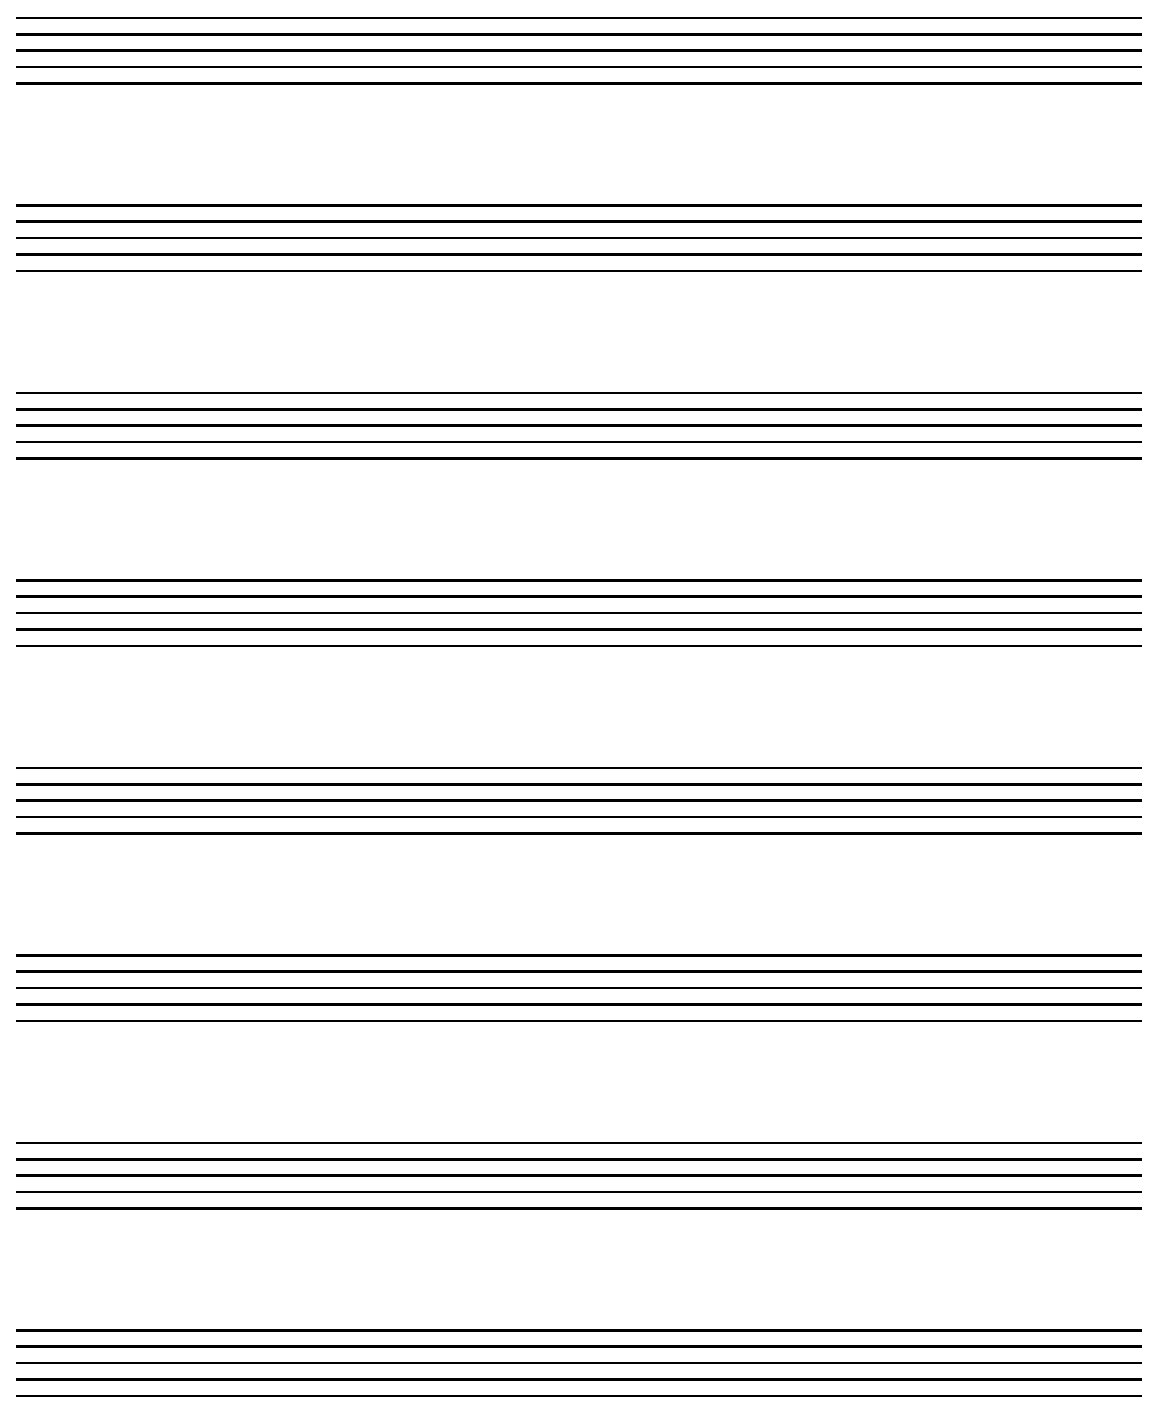
\includegraphics[width=7.5in]{graphics/staves.eps}
\end{figure}

\begin{figure}
\centering
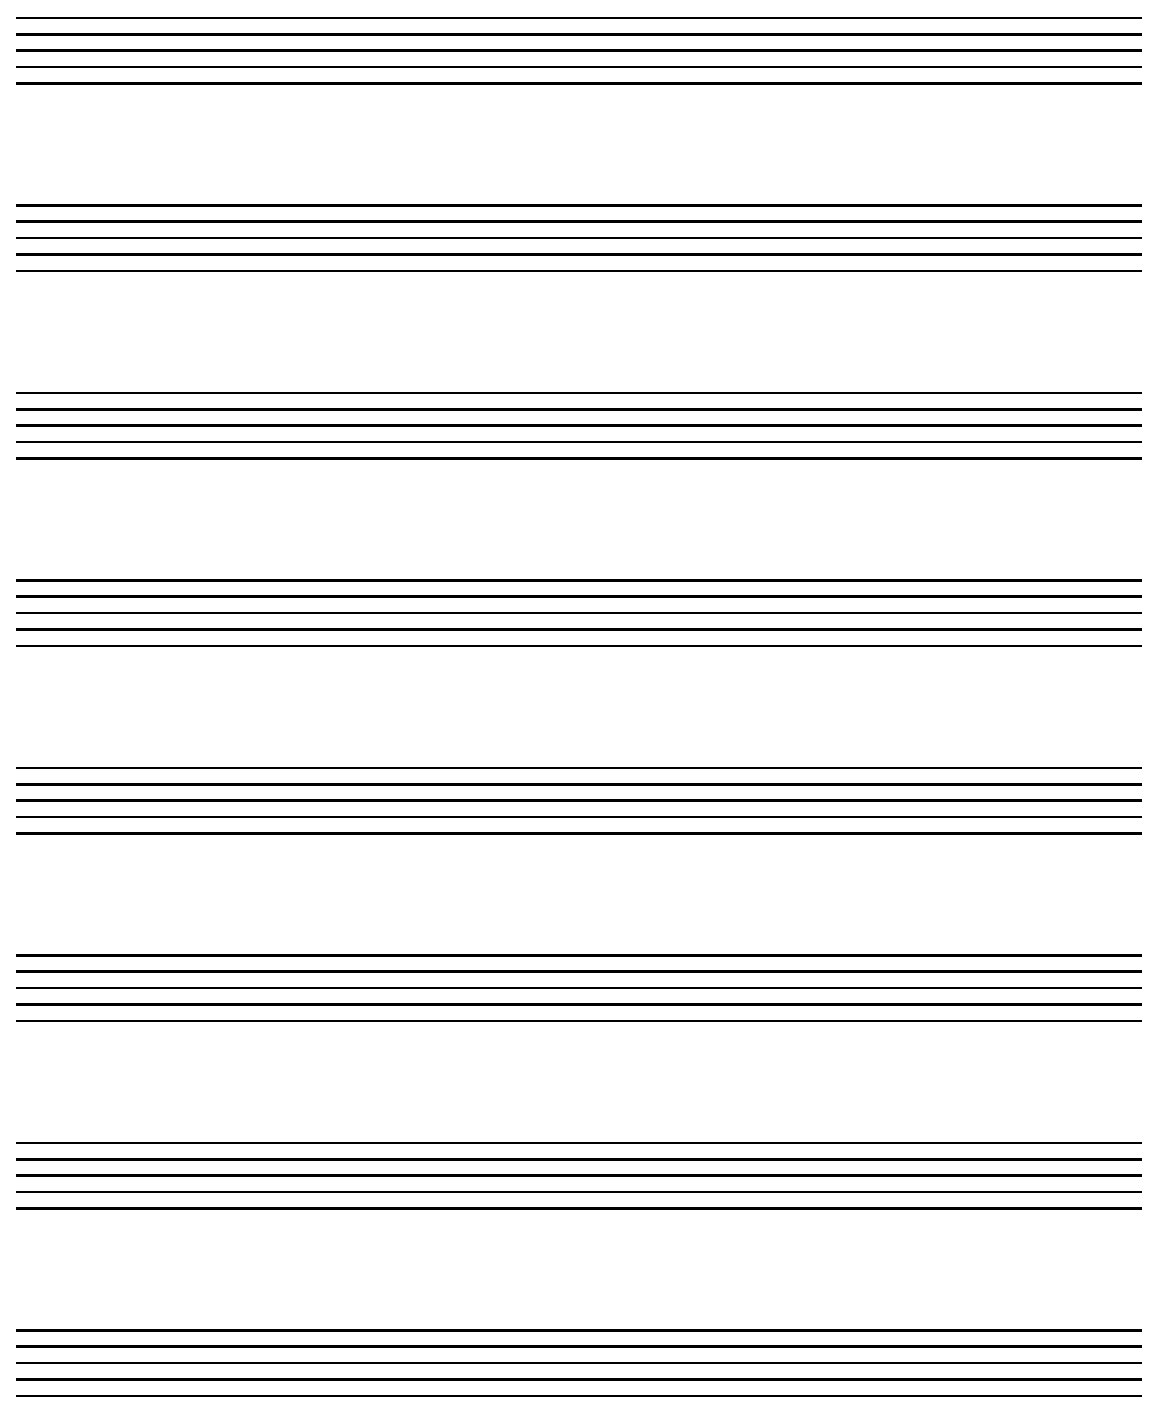
\includegraphics[width=7.5in]{graphics/staves.eps}
\end{figure}

\begin{figure}
\centering
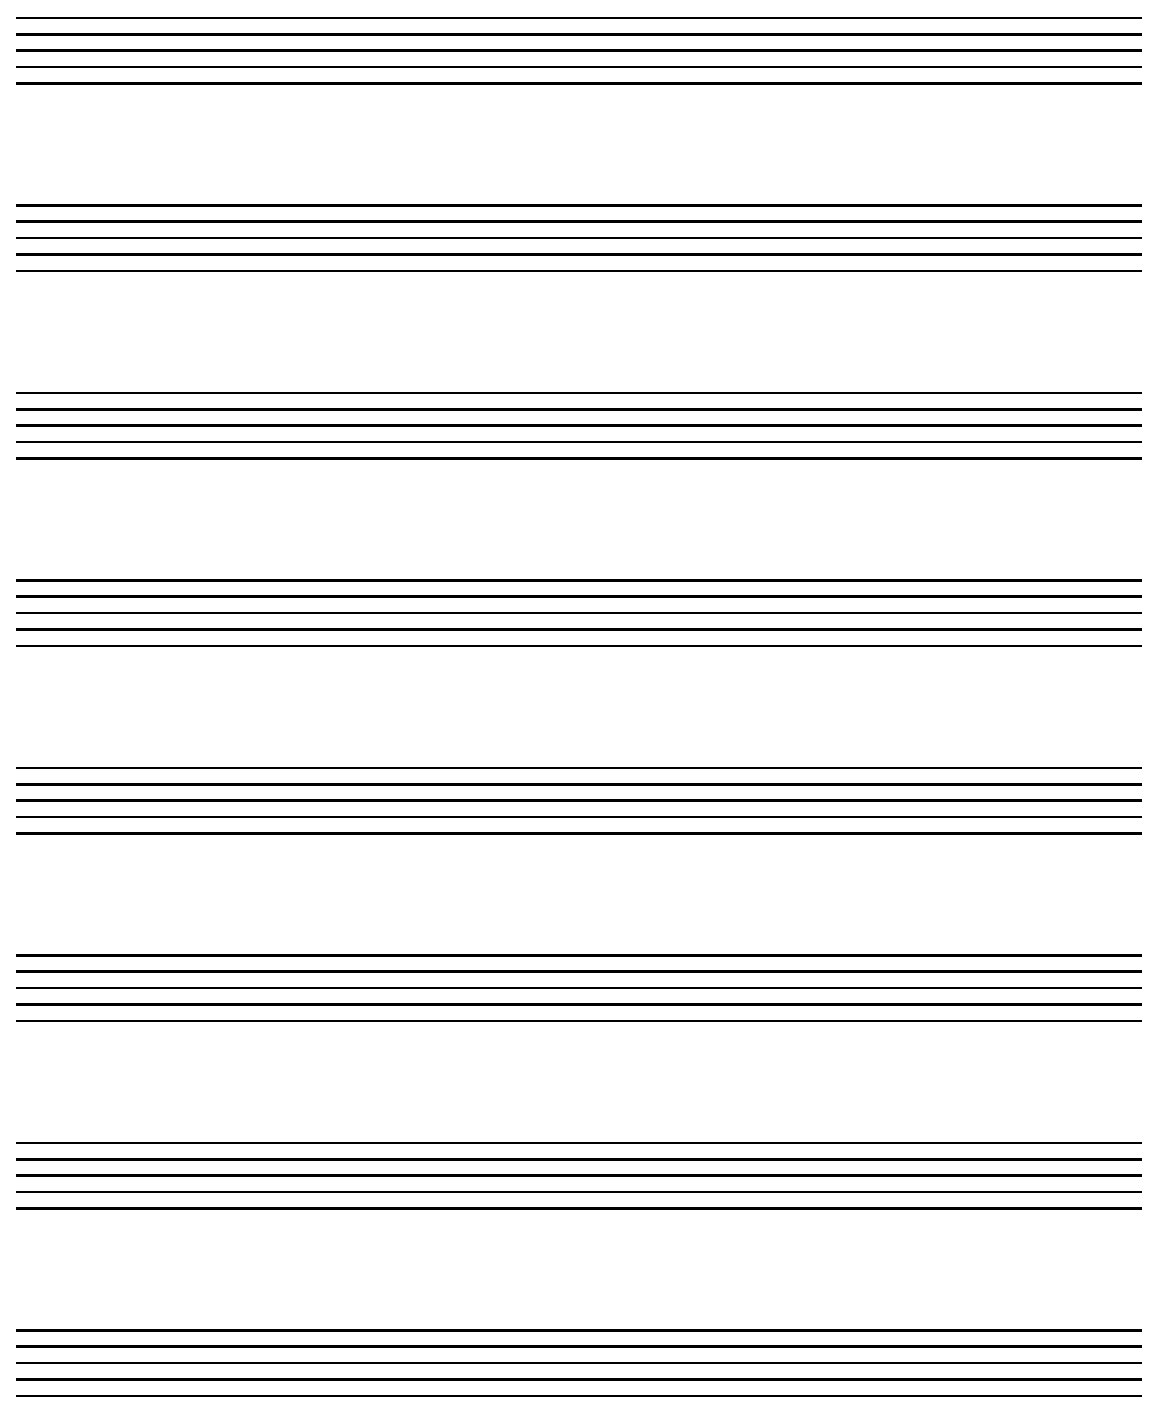
\includegraphics[width=7.5in]{graphics/staves.eps}
\end{figure}

\begin{figure}
\centering
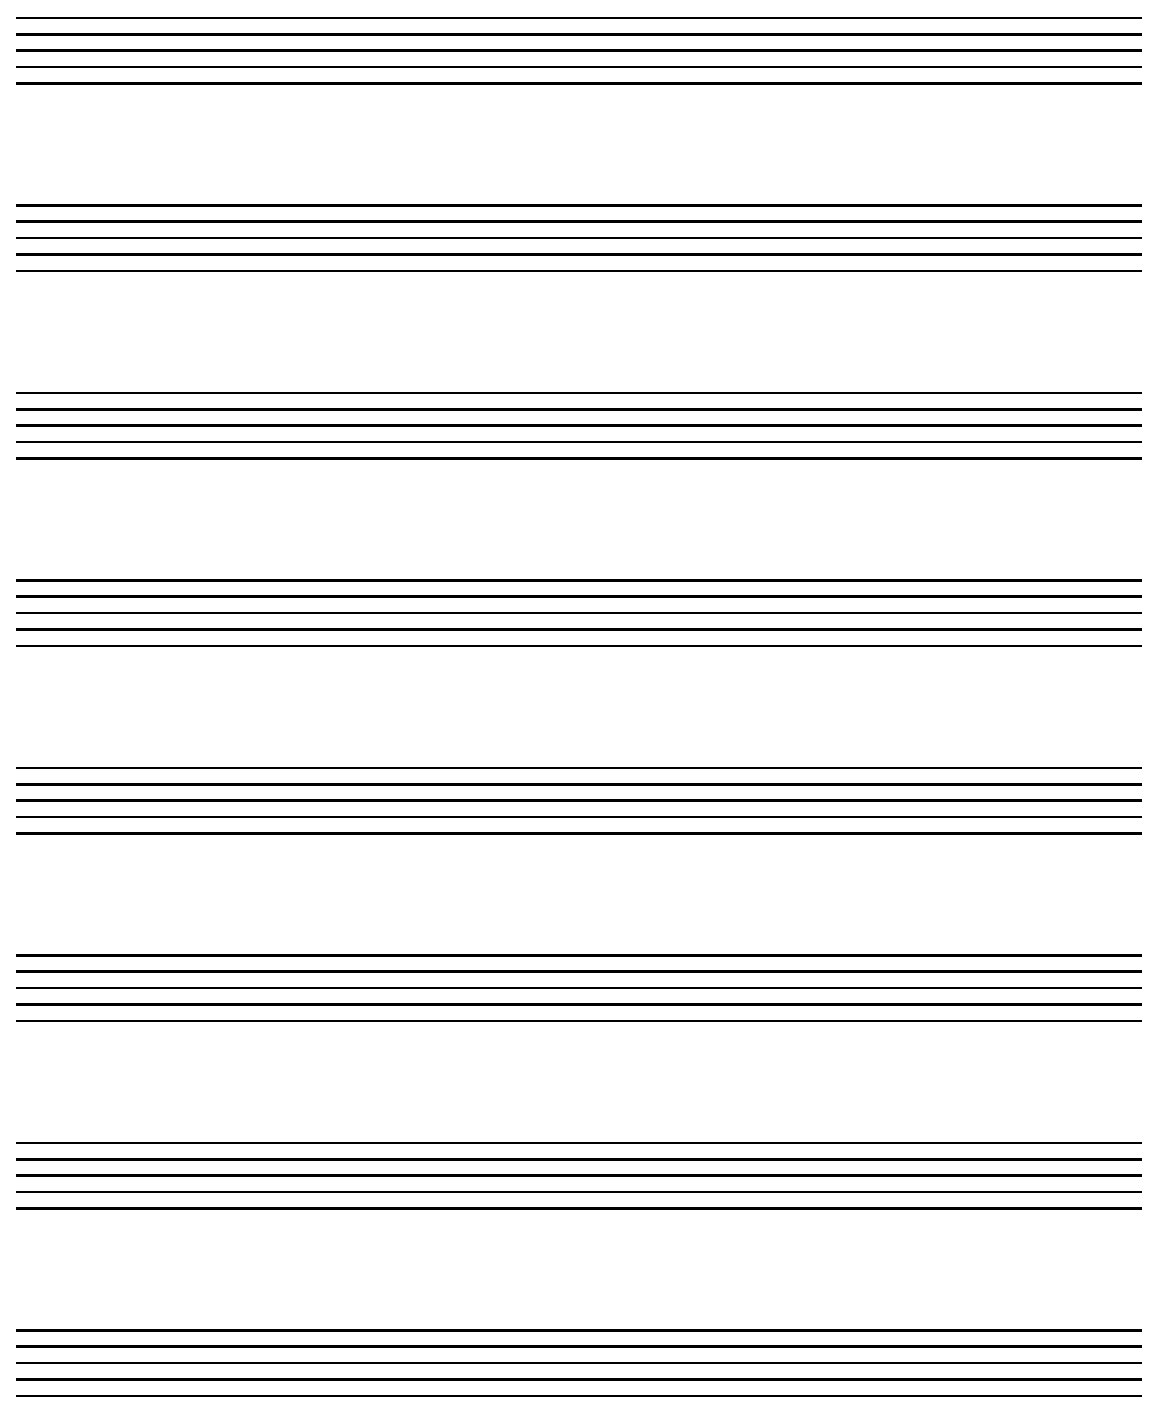
\includegraphics[width=7.5in]{graphics/staves.eps}
\end{figure}

\begin{figure}
\centering
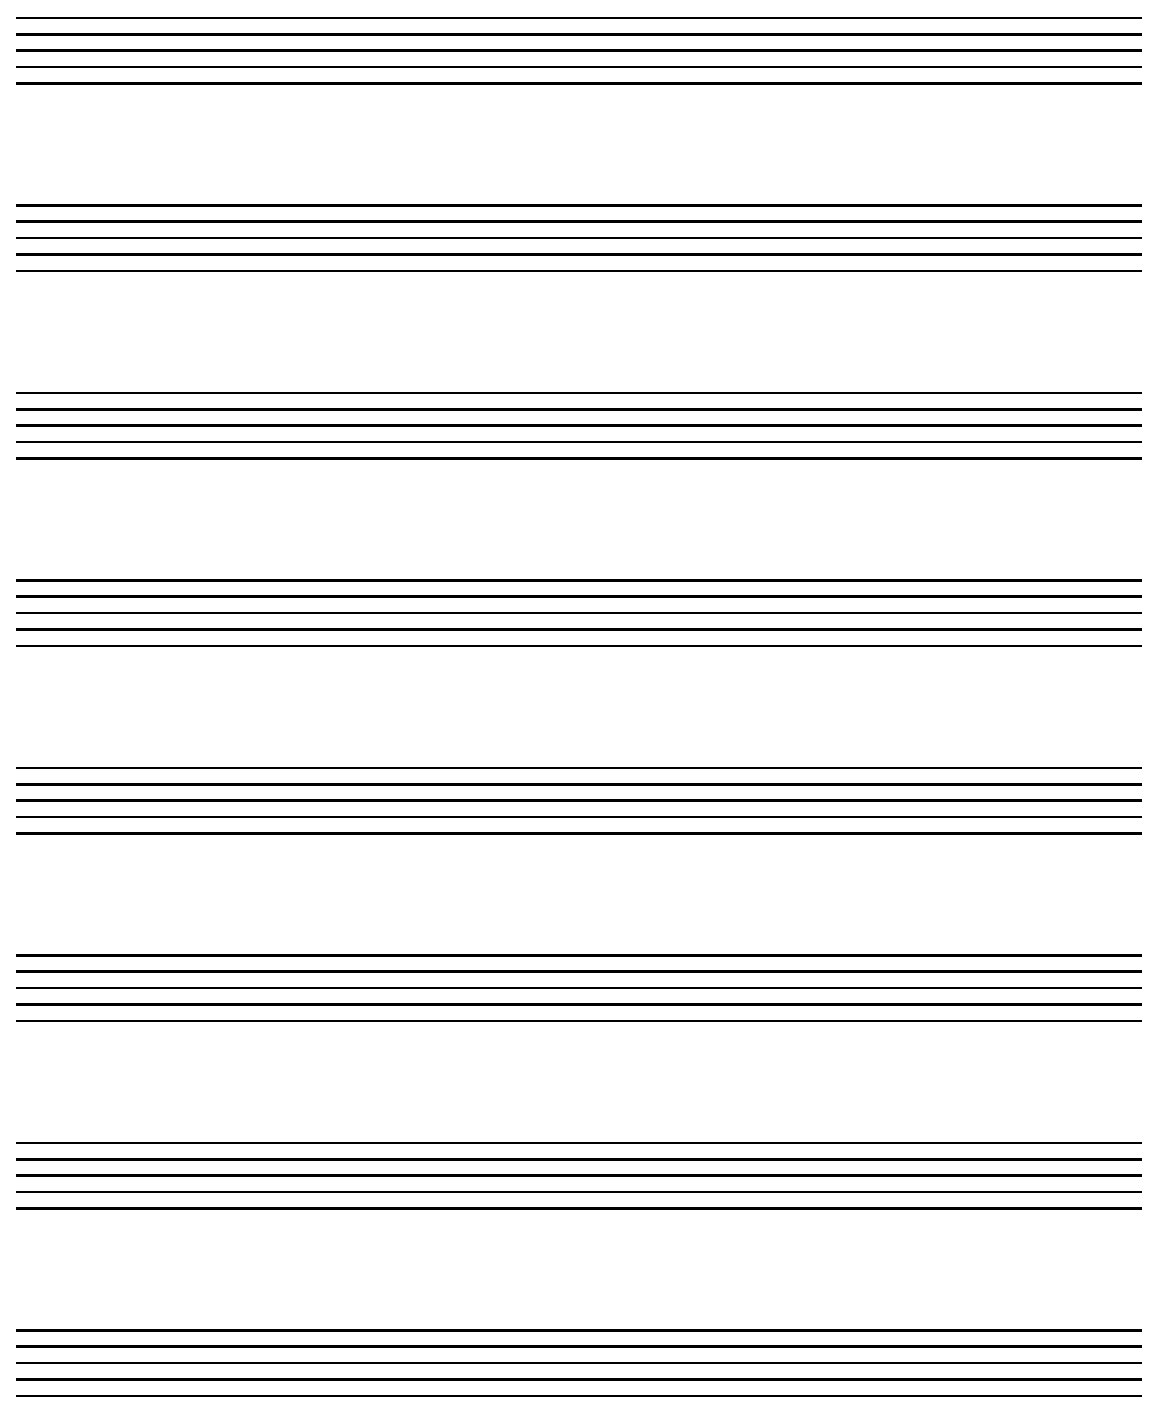
\includegraphics[width=7.5in]{graphics/staves.eps}
\end{figure}


\cleardoublepage


\end{document}
